\documentclass[sisc-eikonal.tex]{subfiles}

\begin{document}

\begin{figure}
  \centering
  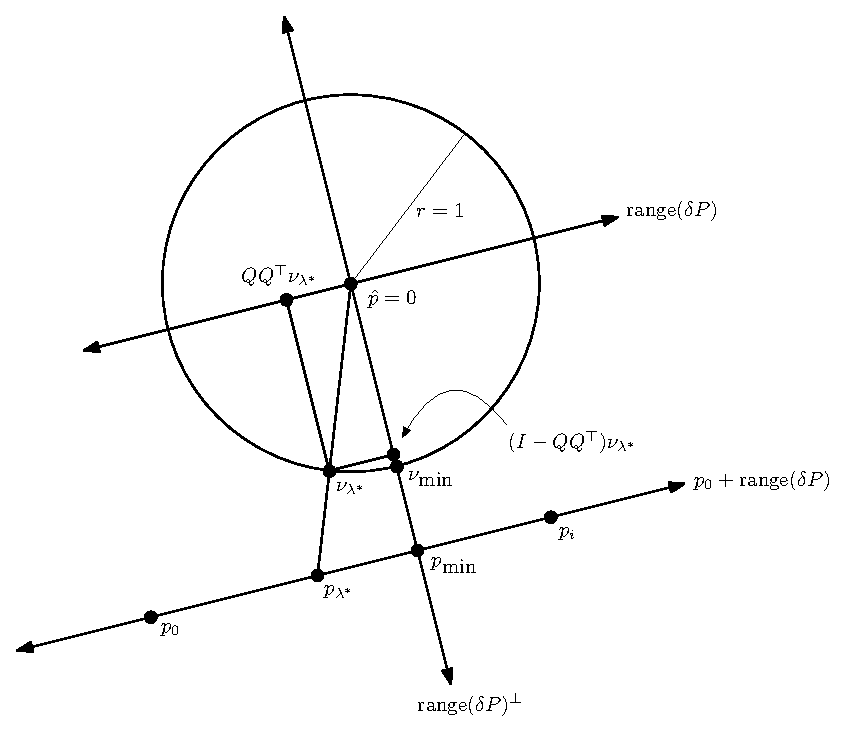
\includegraphics[width=0.65\linewidth]{f0-exact.eps}
  \caption{A schematic depiction of the different quantities involved
    in the proof of \cref{thm:f0-exact}.}\label{fig:f0-exact}
\end{figure}

\section{Proofs for section \ref{ssec:exact-soln}}

\begin{proof}[Proof of \cref{thm:f0-exact}]
  We proceed by reasoning geometrically; \cref{fig:f0-exact} depicts
  the different quantities and the geometric setup. First, with
  $\delta P = QR$, and writing $\nu_{\lambda^*} = p_{\lambda^*}/l_{\lambda^*}$, we
  note that $\lambda^*$ satisfies:
  \begin{equation}\label{eq:Qt-n}
    - R^{-\top} \frac{\delta u}{s^\theta h} = Q^\top \nu_{\lambda^*}
  \end{equation}
  by optimality. Since $QQ^\top$ orthogonally projects onto the span
  of $\delta P$, we can try to write $p_{\lambda^*}$ by splitting it
  into a component that lies in $\range(\delta P)$ and one that lies
  in $\range(\delta P)^\perp$. Letting $\pmin$ be the point in
  $p_0 + \range(\delta P)$ with the smallest 2-norm, we write:
  \begin{equation}\label{eq:plam-decomp}
    p_{\lambda^*} = (p_{\lambda^*} - \pmin) + \pmin,
  \end{equation}
  where $p_{\lambda^*} - \pmin \in \range(\delta P)$ and
  $\pmin \in \range(\delta P)^\perp$. The vector $\pmin$ corresponds to
  $p_{\lambdamin}$ where $\lambdamin$ satisfies:
  \begin{equation}
    0 = \delta P^\top (\delta P \lambdamin + p_0) = R^\top R \lambdamin + R^\top Q^\top p_0,
  \end{equation}
  hence $\lambdamin = -R^{-1} Q^\top p_0$, giving us:
  \begin{equation}\label{eq:pmin}
    \pmin = p_0 + \delta P \lambdamin = {(I - QQ^\top)} p_0.
  \end{equation}
  This vector is easily obtained. For $p_{\lambda^*} - \pmin$, we note
  that $QQ^\top \nu_{\lambda^*}$ is proportional to
  $p_{\lambda^*} - \pmin$, suggesting that we determine the ratio
  $\alpha$ satisfying
  $p_{\lambda^*} - \pmin = \alpha QQ^\top \nu_{\lambda^*}$. In
  particular, from \cref{fig:f0-exact}, we have, using \cref{eq:Qt-n}:
  \begin{equation}\label{eq:alpha-solve}
    \alpha = \frac{\norm{\pmin}}{\norm{(I - QQ^\top) \nu_{\lambda^*}}} = \sqrt{\frac{p_0^\top {(I - QQ^\top)} p_0}{1 - \norm{Q^\top \nu_{\lambda^*}}^2}} = \sqrt{\frac{p_0^\top {(I - QQ^\top)} p_0}{1 - \norm{R^{-\top} \frac{\delta u}{s^\theta h}}^2}}.
  \end{equation}
  At the same time, since
  $\nu_{\lambda^*}^\top (I - QQ^\top) \nu_{\lambda^*} = l_{\lambda^*}^{-2}
  p_0^\top (I - QQ^\top) p_0$, we can conclude that:
  \begin{equation}
    l_{\lambda^*} = \alpha = \sqrt{\frac{p_0^\top {(I - QQ^\top)} p_0}{1 - \norm{R^{-\top} \frac{\delta u}{s^\theta h}}^2}},
  \end{equation}
  giving us \cref{eq:l-star-expression}, proving the first part of
  \cref{thm:f0-exact}.

  Next, combining
  \cref{eq:Qt-n,eq:plam-decomp,eq:pmin,eq:alpha-solve}, we get:
  \begin{equation}\label{eq:plam-final}
    p_{\lambda^*} = {(I - QQ^\top)}p_0 - \sqrt{\frac{p_0^\top {(I - QQ^\top)} p_0}{1 - \norm{R^{-\top} \frac{\delta u}{s^\theta h}}^2}} Q R^{-\top} \frac{\delta u}{s^\theta h}.
  \end{equation}
  This expression for $p_{\lambda^*}$ can be computed from our problem
  data and $\delta P$. Now, note that
  $p_{\lambda^*} = p_0 + \delta P \lambda^*$ implies:
  \begin{equation}\label{eq:lambda-1}
    \lambda^* = R^{-1} Q^\top (p_{\lambda^*} - p_0).
  \end{equation}
  Substituting \cref{eq:plam-final} into \cref{eq:lambda-1}, we obtain
  \cref{eq:f0-exact-lambda} after making appropriate cancellations,
  establishing the second part of \cref{thm:f0-exact}.

  To establish \cref{eq:f0-exact}, we note that by optimality of
  $\lambda^*$, our expression for $\nabla F_0$ (\cref{eq:F0-grad} of
  \cref{lemma:F0-grad-and-Hess}) gives:
  \begin{equation}
    \delta U = -s^\theta h \frac{\delta P^\top p_{\lambda^*}}{l_{\lambda^*}}.
  \end{equation}
  This lets us write:
  \begin{equation}\label{eq:delta-U-dot-lambda-star}
    \delta U^\top \lambda^* = -\frac{s^\theta h}{l_{\lambda^*}} p_{\lambda^*}^\top \delta P^\top \lambda^* = \frac{s^\theta h}{l_{\lambda^*}} p_{\lambda^*}^\top {(p_0 - p_{\lambda^*})}.
  \end{equation}
  Combining \cref{eq:delta-U-dot-lambda-star} with our definition of
  $F_0$ yields:
  \begin{equation}
    \hat{U} = F_0(\lambda^*) = U_0 + \delta U^\top \lambda^* + s^\theta h l_{\lambda^*} = U_0 + \frac{s^\theta h}{l_{\lambda^*}} p_{\lambda^*}^\top {(p_0 - p_{\lambda^*})} + \frac{s^\theta h}{l_{\lambda^*}} p_{\lambda^*}^\top p_{\lambda^*},
  \end{equation}
  which gives \cref{eq:f0-exact}, completing the final part of the
  proof.
\end{proof}

\end{document}

%%% Local Variables:
%%% mode: latex
%%% TeX-master: "<none>"
%%% End:
